\iffalse
\documentclass[10pt, a4paper]{article}
\usepackage[a4paper,outer=1.5cm,inner=1.5cm,top=1.75cm,bottom=1.5cm]{geometry}

\twocolumn
\usepackage{graphicx}

\usepackage{hyperref}
\usepackage[utf8]{inputenc}
\usepackage{amsmath}
\usepackage{physics}
\usepackage{amssymb}
\begin{document}
\title{Assignment-4}
\author{Name:A.SUSI\and Email :  \url{susireddy9121@gmail.com}}
%\{ Wireless Communication (FWC)}
\date{30-sep-2022}
\maketitle



\section{Problem}
\fi
\solution 
\iffalse
\section{Solution}
\begin{center}
The input given 
\boldmath
\fi 
Let
\begin{align} 
\vec{A}=\myvec{ h\\ 0 },
\vec{B}=\myvec{ a\\ b },
\vec{C}=\myvec{ 0\\ k }
\end{align}
Forming the matrix in 
	\eqref{eq:normal_line-collinear}, we obtain, upon row reduction
	\iffalse
\begin{align}
\myvec{ h-a & -b\\ h & -k  } 
\end{align}
Using row reduction, 


In the problem they have given that three points lie on a line, thats means these three points are collinear.\\
If  points on a line  are  collinear, rank of matrix is "1"then the vectors are in linearlydependent.\\
For 2 × 2 matrix Rank =1 means Determinant is 0.\\
Through pivoting,we obtain\\
\fi
\begin{align}\label{eq:}
\myvec{ h-a & -b\\ h & -k  }  
	\xleftrightarrow[]{{\frac{R_1}{h-a}}}\myvec{
1 &\frac{-b}{h-a} \\ 
 h& -k
}
	\\
	\xleftrightarrow[]{R_2\rightarrow R_2-hR_1}
\myvec{
1 &\frac{-b}{h-a} \\ 
 0&-k+\frac{bh}{h-a} 
}
\end{align} 
For obtaining a rank 1 matrix, 
\iffalse

if the rank of the matrix is 1 means any one of the row must be zero.So, making the last element in the matrix to 0.\\
\fi
\begin{align}
	-k+\frac{bh}{h-a}&=0
	\\
	\implies \frac{a}{h}+\frac{b}{k}&=1 
\end{align} 
upon simplification.
\iffalse

Hence proved.\\
\section{Construction}
 \begin{figure}[h]
\centering
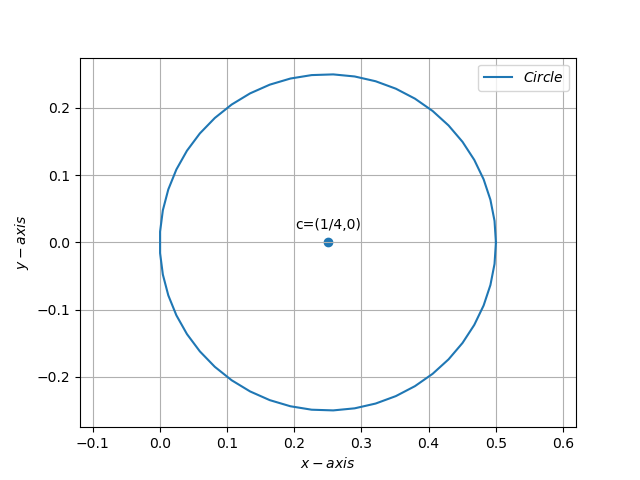
\includegraphics[scale=0.4]{fig.png} 
\caption{}
\end{figure}
\section{Code}
*Verify the above proofs in the following code.\\
\framebox{
\url{https://github.com/Susi9121/FWC/tree/main/matrix/line}}	
\bibliographystyle{ieeetr}
\end{document}
\fi
